\chapter{Analisi dei requisiti}
\section{Ideazione}
La maggior parte dei progetto richiede un breve passo iniziale in cui
si esaminano i seguenti tipi di domande:
\begin{itemize}
    \item Il progetto è fattibile?
    \item Comprare e/o costruire?
    \item Stima approssimativa e non affidaivbile dei costi
    \item Dovremmo procedere o fermarci?
\end{itemize}
L'ideazione non è la fase dei requisiti.
\\ Il problema principale che risolve l'ideazione è il seguente:
\begin{center}
    \textbf{Le parti interessate hanno un accordo di base, sulla visione
    del progetto, e vale la pena di investire un'indagine seria?}
\end{center}
Lo scopo è quindi quello di stabilire una visione comune per gli obiettivi del progetto
e capire se questo è fattibile.
\\ In questa fase non si utilizza molto UML (verrà utilizzato soprattutto durante
 l'elaborazione).
\paragraph*{Non hai capito l'ideazione se}
\begin{itemize}
    \item Dura più di qualche settimana
    \item Provi a definire molti requisiti
    \item Ci si aspetta che i piani e le stime siano affidabili
    \item I nomi di molti attori e casi d'uso non sono stati identificati
    \item Troppi casi d'uso sono stati scritti nel dettaglio
    \item Nessun caso d'uso è stato scritto in dettaglio
\end{itemize}
\section{Che sono sono i requisiti}
Un requisito è una capacità o una condizione a cui il sistema e più in generale il
progetto, deve essere conforme.
\\ I requisiti sono un aspetto veramente molto importante, si evidenzia
addirittura che 34 \% delle cause dei fallimenti dei progetti software
riguardano l'attività dei requisiti.
\paragraph*{Ci sono due tipi principali di requisiti}
\begin{itemize}
    \item Requisiti funzionali (comportamentali) - Descrivono il comportamento del
    sistema, in termini di funzionalità fornite ai suoi utenti e informazioni
    che il sistema deve gestire
    \item Requisiti non funzionali (tutti gli altri requisiti) - Sono relativi
    a proprietà del sistema nel suo complesso come per esempio sicurezza, presetazioni,
    scalabilità, usabilità...
\end{itemize}
\subsection{Requisiti funzionali}
Sono funzionalità o servizi che il sistema deve fornire, risposte che l'utente
aspetta dal software in determinate condizioni, risultati che il software deve produrre
in risposta a specifici input.
\paragraph{Il problema dell'imprecisione nella specifica dei requisiti}
Requisiti ambigui possono portare a diverse interpretazioni da sviluppatori e utenti.
In linea di principio i requisiti dovrebbero essere completi e coerenti, quindi
includere la definizione di tutti i servizi richiesti e non essere ambigui.
\subsection{Requisiti non funzionali}
questi definiscono le proprietà e i vincoli del sistema, ad esempio affidabilità,
tempi di risposta, oppure vincoli come la capacità dei dispositivi I/O,
le rappresentazioni dei dati nelle interfacce di sistema, ecc.
\\I requisiti funzionali possono essere più critici dei requisiti funzionali, in caso
contrario il sistema potrebbe risultare inutilizzabile.
\paragraph*{Obiettivi e requisiti} I requisiti non funzionali possono essere molto
difficili da stabilire con precisioni e requisiti imprecisi possono essere
difficili da verificare.
\\ Un obiettivo può essere un intenzione generale dell'utente come la facilità d'uso,
mentre un requisito non funzionale verificabile è una dichiarazione che utilizza
alcune misure oggettivamente verificabili.
Gli obiettivi sono utili agli sviluppatori in quanto trasmettono le intenzioni degli
utenti del sistema.
\paragraph*{Metriche per specificare i requisiti non funzionali}
\begin{center}
    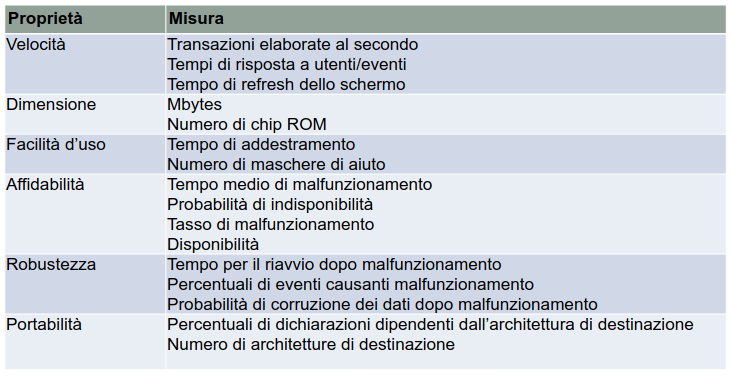
\includegraphics[width=100mm, scale=0.5]{metriche_requisiti_non_funzionali.png}
\end{center}
